\section{Introduction}
The developed methodology accounts for performance characteristics in a concise way that lends itself to optimization formulation without becoming intractable. This chapter discusses the relevance of the aircraft routing problem in literature as well as their shortcomings with respect to the inclusion of aircraft performance. Additionally, the chapter introduces several formulations in which the methodology is used to account for fuel efficiency and loiter availability at interest locations. The first two formulations explore the use of the methodology with multiple aircraft interested in traveling to multiple locations and optimizing total loiter time and priority of locations. The last formulation examines the inclusion of fuel burn on a single aircraft's path to multiple locations while loitering at each location.
\section{Aircraft Routing Optimization Literature Review}
The aircraft assignment problem is an application of the assignment problem to target locations from a starting point. A modified assignment problem can consist of one aircraft and multiple locations, a one-to-one matching of aircraft to target locations, or multiple aircraft to a greater number of locations. An assignment problem is a special case of the transportation problem where supply and demand are equal to one for all locations. The mathematical model for an assignment problem is as follows:
\begin{align}
    \min\hspace{0.5cm} &\sum_{i=1}^m\sum_{j = 1}^mc_{ij}x_{ij}\\
    \text{s.t.} \hspace{0.5cm} &\sum_{j=1}^mx_{ij} = 1, \hspace{0.5cm} \forall i \in \{1,...,m\}\\
    &\sum_{i=1}x_{ij} = 1, \hspace{0.5cm} \forall j \in \{1,...,m\}\\
    &x_{ij} \in \{0,1\}, \hspace{0.5cm} \forall i,j\in \{1,...,m\}
\end{align}
where $c_{ij}$ is the cost of assigning $i$ to $j$ and $m$ is the number of assignments \cite{bazaraa}. 
\par
A binary integer linear program (BIP) is generally the designation of assignment problems, given that the constraints and objective function are linear and that an assignment decision variable is binary-valued. In their paper on the UAV routing assignment problem, Shetty et al. \cite{Shetty} use a mixed integer linear program wherein the main constraints are service level and weaponry constraints. Their formulation serves as a traveling salesman problem (TSP), where the objective is to minimize cost, but all locations must be visited in the model. There is no upper-level constraint for ability to travel or service for any amount of time. While this formulation showcases a valid assignment problem for UAV waypoints and is similar to the way a formulation for multiple aircraft waypoints are visited, the constraints do not capture the performance characteristics of the aircraft and only seek to minimize cost rather than matching realistic performance capabilities. \par
In contrast, Alighanbari et al. \cite{Alighanbari}, Schumacher et al. \cite{Schumacher}, and Taylor et al. \cite{Taylor}, use constrained optimization based on range, timing, or fuel ratios. The advantage of this formulation is that it can represent real-world scenarios such as UAV waypoints \cite{Alighanbari} or flight mapping for commercial airliners \cite{Taylor}. Although Taylor et al. \cite{Taylor} used the TSP formulation in their model, the idea of using fuel as a constraint accounts for all possible maneuvers in an aircraft. This formulation informs the way performance characteristics of the aircraft is accounted for within constraints.\par
Vitte \cite{OptimizeBreguet} discusses the continuous coverage of a target area using a time on station designation and assuming a constant idle time. His formulation allowed for a maximization of time on station for a certain number of aircraft while meeting the constraints for turn-around time and outbound time for any particular aircraft. Integrating this idea while allowing for multiple target locations in an imperfect matching scheme allows for a decision maker to maximize the priority of targets with limited resources. While this is promising with respect to maximizing the priority of targets, the formulation lacks relevance to the performance characteristics of the aircraft used and disregards the fuel efficiency of an aircraft as it burns fuel.\par
Kannon et. al. \cite{Kannon} examines the incorporation of fuel over a series of time steps in an aircraft routing formulation. At each time step, fuel can change depending on a previous aerial refueling. Using an MILP, the formulation solves for the optimal optimal route through a series of intermediary nodes and the refueling intermediary node between a source and sink. The concept of a time step can follow the use of fuel along a route and involve how fuel efficiency changes over fuel burn. This formulation informs the way fuel is initialized as a decision variable and constrained over the course of the solution process.\par

%Missing from the lit review is how the works relate (or don't) to your own. At present, a reader doesn't know why each work is reviewed.  For a given work, is it foundational in some way?  Does it inform your model?  Does it inform your conceptual development of a model?  Or was it a promising approach that didn't quite fit your problem, so it's important to indicate how your problem differs in a way that requires a different model?
\section{Initial Formulation}
Let $x_{ij}$ be a binary variable where $x_{ij} = 1$ if plane $i$ travels to location $j$. Additionally let $d_{ij}$ be the number of miles from a starting, $i$ point to an interest location,$j$, and $E_{ij}$ be the maximum loiter time, given that aircraft $i$ has traveled to location $j$ where is calculated using Eq. \ref{eq:EnduranceWithRange} with $d_{ij}$ used as the range. A negative number in the $E_{ij}$ represents an inability for the aircraft to reach location $j$ from location $i$ and results in a penalty to the overall objective function. The sets $I$ and $J$ are represented as $I = \{1,2,\dots,n\}$ and $J = \{1,2,\dots,m\}$ where $n$ is the number of aircraft and $m$ is the number of locations. The formulation for maximizing endurance with $n$ aircraft and $m$ locations follows.\par

\begin{align}
    \max &\sum_{i\in I}\sum_{j\in J} E_{ij}x_{ij}\hspace{1cm}\\
    \text{s.t } &\sum_{i\in I} x_{ij}\leq 1\hspace{1cm} \forall j\in J\\
    &\sum_{j\in J}x_{ij} \leq 1\hspace{1cm} \forall i \in I\\
    &x_{ij}\in \{0,1\} \hspace{1cm} \forall i\in I, j\in J
\end{align}
The constraints represent a typical transportation problem where each aircraft can travel to at most one location and each location can be visited once. Using the Haversine formula and the methodology described in Section \ref{section:havMethod}, the endurance matrix is determined for an aircraft's performance parameters. \par
\section{Priority Assignment Formulation}
The priority assignment formulation is similar to the initial formulation and allows prioritizing locations. The decision for an interests point's priority is defined by the vector $\mathbf{v}$. The formulation for maximizing endurance with $n$ aircraft and $m$ locations follows.\par
\begin{equation}
    \begin{aligned}
        \max &\sum_{i\in I}\sum_{j\in J} E_{ij}v_{j}x_{ij}\hspace{1cm}\\
        \text{s.t } &\sum_{i\in I}x_{ij} \leq 1,\hspace{1cm} \forall j\in J,\\
        &\sum_{j\in J}x_{ij} \leq 1,\hspace{1cm} \forall i \in I,\\
        &x_{ij}\in \{0,1\}, \hspace{1cm} \forall i\in I, j\in J.
    \end{aligned}
\end{equation}
Though $v_j$ in this case is represented as a discrete matrix of priorities, there can also be a distribution with the endurance associated with an interest location. This broadens the ability of this formulation to utilize the developed methodology for incorporating the dynamic flight characteristics of aircraft into an assignment decision rather than a static constraint used in other literature \cite{Alighanbari,Schumacher,Taylor}.
\section{Assignment Problem Tests}
The assignment problem was tested using the aircraft parameters from AC4-000. Although the AC4-000 stressed the proposed method and incurred the most error and had the most conservative estimate from the current method, this aircraft had the longest range and, with the given list of interest points, found non-trivial solutions. The combat fuel and climb fuel were set to zero to assume that the aircraft was only interested in loiter at its respective location. The interest points were a random sequence of 100 cities in the US. All tests were run on the same 100 cities. \par
The sample problem assigned an arbitrary number of twenty aircraft to visit twenty nodes to meet the objective of maximizing total endurance. Figure \ref{fig:trivialAP} shows the results of the optimization problem run using the SCIP solver \cite{scip}.\par
\begin{figure}[H]
    \centering
    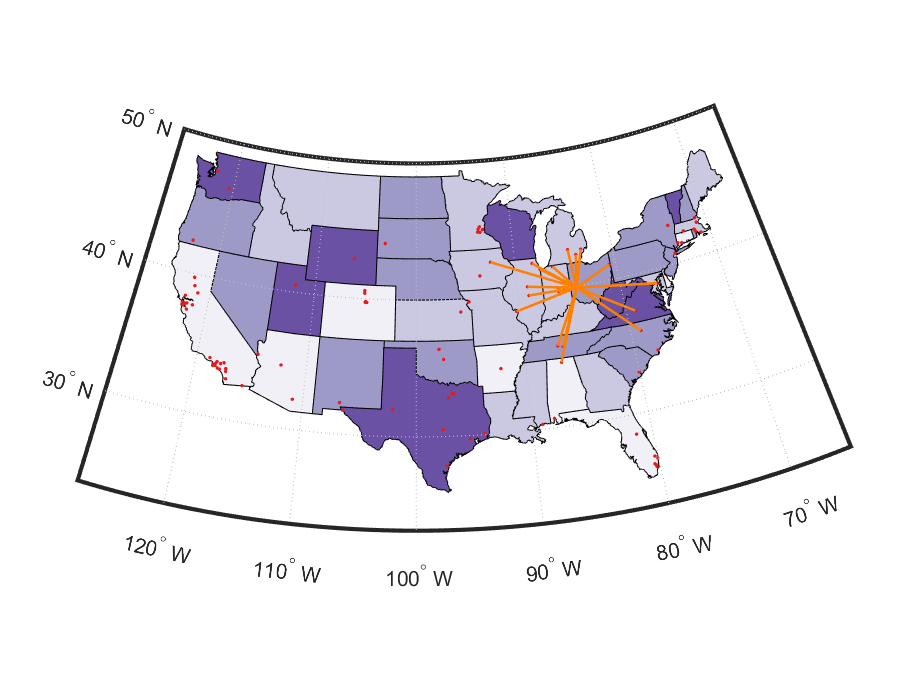
\includegraphics{Thesis/Method_II/trivialAP.eps}
    \caption{Initial Assignment Problem Example}
    \label{fig:trivialAP}
\end{figure}
As hypothesized, the results show a relatively trivial solution since all aircraft are the same and endurance at all locations is weighted equally. The twenty aircraft were assigned to the twenty nearest locations.\par
The priority assignment problem assigned a random priority to each location between zero and twenty. This test was in an attempt to determine whether a non-trivial solution can be found when certain locations are more desirable to endure over than others. The same aircraft and locations were used in this problem as in the initial assignment problem example. Figure \ref{fig:priorityAP} shows the results of the optimization problem run using the SCIP solver \cite{scip}.
\begin{figure}[H]
    \centering
    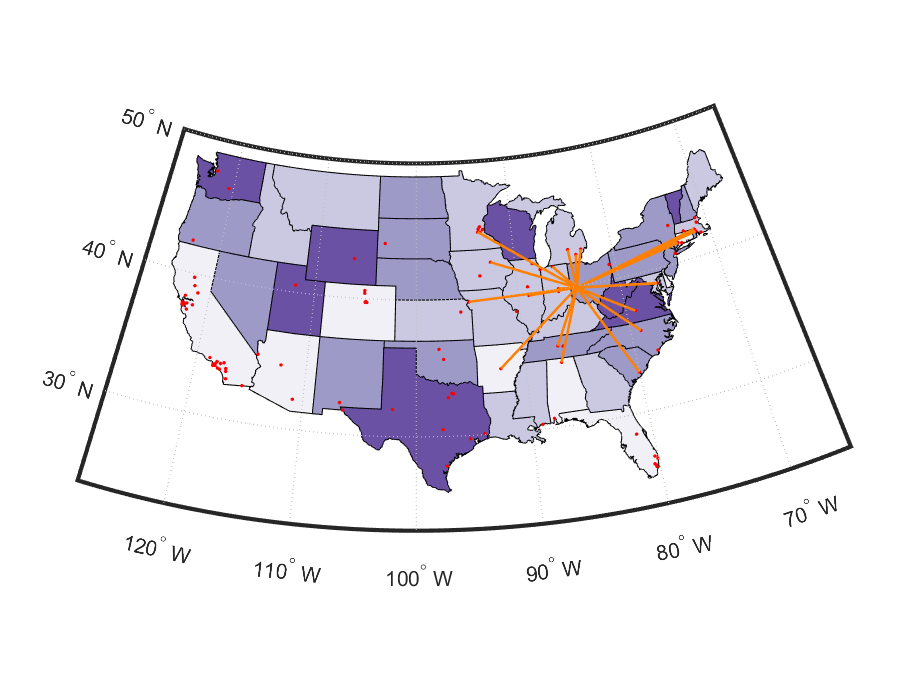
\includegraphics{Thesis/Method_II/priorityAP.eps}
    \caption{Priority Assignment Problem Example}
    \label{fig:priorityAP}
\end{figure}
The optimization problem solution verified that certain locations were a higher priority than others despite the decreased available loiter time. The aircraft traveled to locations past the previous solutions interest locations and chose to loiter at these interest points due to their higher interest.\par
Using the same optimization formulation as the priority assignment formulation, the last test was using four different aircraft, the F-15C, AC2-000, AC3-000, and AC4-000. Since these three have different endurance capabilities at their given parameters in Table \ref{tab: aircraft parameters}, the problem seeks to maximize priority while balancing the dynamic characteristics of the different aircraft. Twenty aircraft were used with five aircraft from each aircraft class. Figure \ref{fig:diffStructuresAP} shows the results of the optimization problem run using the SCIP solver \cite{scip}.
\begin{figure}[H]
    \centering
    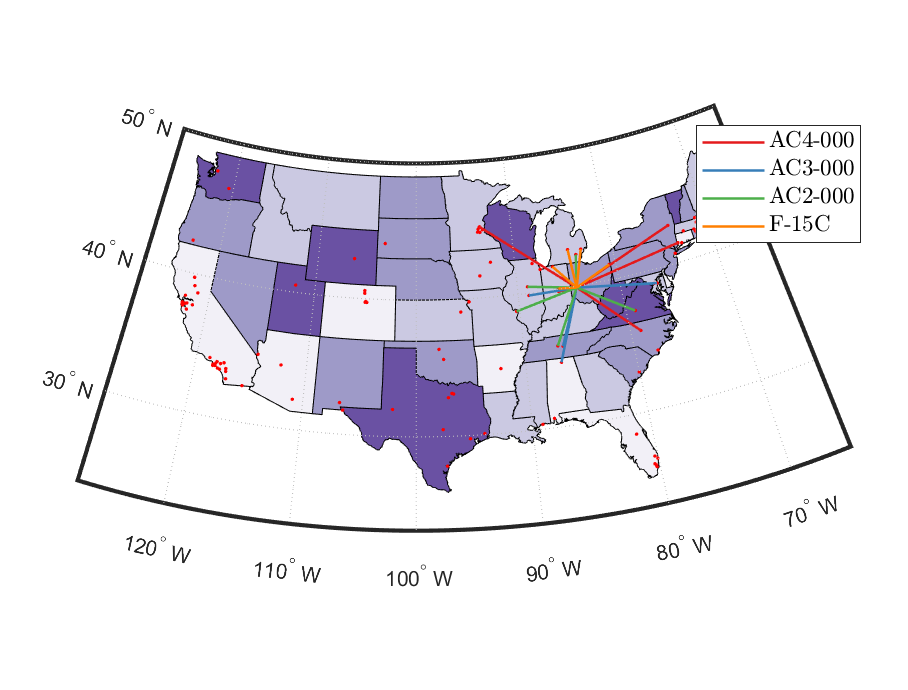
\includegraphics{Thesis/Method_II/diffStructuresAP.eps}
    \caption{Different Structures Example (with Random Priority)}
    \label{fig:diffStructuresAP}
\end{figure}
The solution showed that the aircraft with the longest range were assigned to the interest locations having both higher priorities and farther locations (AC4-000) and the shorter range aircraft were assigned to loiter over the closer distances. \par 
The assignment problem formulations successfully leveraged the methodology to quickly find a maximum loiter time over any interest location using the flight characteristics of each aircraft and in turn solve an assignment problem that maximized the interest location preferences. The solution to the priority assignment formulations were non-trivial and partitioned priority with loiter time and aircraft abilities.

\section{Decision Dependent Formulation}
\label{section:DDF}
This sub-problem seeks to route an aircraft with the given flight characteristics to multiple locations while incorporating the fuel efficiency of the nonlinear Br\'eguet range equation. The aircraft must always start from a given source node and may visit any connected node, given that the move is feasible according to its flight characteristics. The following set of parameters, decision variables, sets, and constraints define the backbone of the mixed integer nonlinear program (MINLP).
\subsection*{Parameters}
\begin{itemize}
    \item $m$ is the number of locations available to travel
    \item $D$ is a matrix of the distances between each point $D\in \mathbf{R}^{m\text{x}m}$
    \item $E$ is a matrix of efficiency factors calculated using Br\'eguet's range equation such that $E_{ij} = \exp\left[\dfrac{-D_{ij}}{V}\dfrac{TSFC}{C_L/C_D}\right]$ and $E\in \mathbf{R}^{m\text{x}m}$
    \item $s$ is both the source and sink of the model
\end{itemize}
\subsection*{Decision Variables}
\begin{itemize}
    \item $x_{ij}^{\tau}$ equals one if the aircraft travels from location $i$ to location $j$ at time decision step $\tau$
    \item $F^{\tau}$ is the amount of fuel used at decision step $\tau$
\end{itemize}
\subsection*{Sets}
\begin{itemize}
    \item $T = \{1,2,...,m\}$
    \item $I = \{1,2,...,m\}$
    \item $J = \{1,2,...,m\}$
\end{itemize}
\subsection*{Constraints}
%$\max \hspace{0.5cm} \sum \text{Endurance Utility (ie logistic curve of: $\sum(f_{ij}-R_{ij}$))}$
\begin{align}
&\sum_{j\in J} x_{sj}^{\tau} = \begin{cases} 
1, & \tau = 1,\\
0, & \forall\tau\in T-\{1\}, \end{cases} \label{cons:comefromsource}\\
&\sum_{j\in J} x_{ij}^{\tau+1}-\sum_{j\in J}x^{\tau}_{ji} = 0, \hspace{0.5cm} \forall i\in N-\{s\},\tau \in T, \label{cons:outtoin}\\
&\sum_{i\in I}x_{ii}^{\tau} = 0, \hspace{0.5cm} \forall \tau \in T, \label{cons:self}\\
&\sum_{i\in I}\sum_{\tau\in T} x_{ij}^\tau\leq 1, \hspace{0.5cm} \forall j \in J,\label{cons:do not revisit}\\
&\sum_{\tau\in T}\sum_{i\in I} x_{is}^\tau = 1,\label{cons:return}\\
&W_F-\left(\sum_{i\in I}\sum_{j\in J}E_{ij}W_Fx_{ij}^1\right) \leq F^{1}, \label{cons:fuelstart}\\
&W_F\sum_{i\in I}\sum_{j\in J}x_{ij}-\left(\sum_{i\in I}\sum_{j\in J}E_{ij}(W_F-\sum_{k = 1}^{\tau}F^{k-1})x_{ij}^{\tau}\right) \leq F^{\tau}, \hspace{.5cm} \forall \tau \in T-\{1\},\label{cons:fuelnext}\\
&\sum_{\tau\in T}\sum_{i\in I}\sum_{j\in J} F^{\tau} \leq F_{total},\label{cons:fueltotal}\\
&x_{ij}^{\tau}\in \{0,1\}, \hspace{0.5cm} \forall i\in I,j\in J,\tau\in T\label{cons:binary}.
\end{align}
Constraint \eqref{cons:comefromsource} accounts for the aircraft originating from the source node at the first decision step. Constraint \eqref{cons:outtoin} only allows the aircraft to depart from the node to which it arrived in the last decision step for all nodes except the source node since the return decision step is not known. Constraint \eqref{cons:self} does not allow the aircraft to travel to the same node at any decision step while constraint \eqref{cons:do not revisit} assures that an aircraft never departs the same node more than once in its route.  Constraint \eqref{cons:return} requires the aircraft to return to the source (once only). Constraints \eqref{cons:fuelstart} and \eqref{cons:fuelnext} incorporate the fuel burn at the start of the maneuver and for each decision step until returning to the source. Decision variable, $F^{\tau}$, is the fuel needed for the range and the additional fuel used for loiter. The variable is constrained by the aircraft's fuel burn from previous steps and needed fuel for the range given its current weight. Constraint \eqref{cons:fueltotal} ensures that the aircraft does not take a route that requires more fuel than it has in it's tank. Lastly, constraint \eqref{cons:binary} restricts the model to binary routing decisions. The nonlinearity of constraint \eqref{cons:fuelnext} differs from the typical MILP in that it requires specialized software or customized algorithms to assure that a global optimal solution is attained.\par
The objective of the decision dependent formulation is malleable in that it depends on the importance of visiting a number interest locations versus the loiter time over each interest location. Either objective can be constrained in an $\varepsilon$-constrained formulation to require a certain number of visited locations and/or a certain amount of loiter time. The former bound is the simplest constraint to implement; where the sum total of all dimensions of $x$ may be required to be greater than or equal to the number of locations. The latter bound is a harder constraint to capture in a linear form without estimating fuel burn for a certain loiter time without accounting for change in weight. A nonlinear formulation would be the most appropriate constraint for a realistic, small model, but a similar result can be obtained by constraining the minimum amount of loiter time spent at a certain location. In the next formulation, the minimum amount of fuel used for loiter time is specified by $f_{min}$.

\begin{align}
\max \hspace{0.5cm} & \sum_{\tau\in T}\sum_{i\in I}\sum_{j\in J}x_{ij}^\tau\\
\text{s.t.}\hspace{0.5cm}&\sum_{j\in J} x_{sj}^{\tau} = \begin{cases} 
1, & \tau = 1,\\
0, & \forall\tau\in T-\{1\}, \end{cases} \\
&\sum_{j\in J} x_{ij}^{\tau+1}-\sum_{j\in J}x^{\tau}_{ji} = 0, \hspace{0.5cm} \forall i\in N-\{s\},\tau \in T, \\
&\sum_{i\in I}x_{ii}^{\tau} = 0, \hspace{0.5cm} \forall \tau \in T, \\
&\sum_{i\in I}\sum_{\tau\in T} x_{ij}^\tau\leq 1, \hspace{0.5cm} \forall j \in J,\\
&\sum_{\tau\in T}\sum_{i\in I} x_{is}^\tau = 1,\\
&W_F-\left(\sum_{i\in I}\sum_{j\in J}E_{ij}W_Fx_{ij}^1\right) - F^{1}\leq -f_{min}, \\
&W_F\sum_{i\in I}\sum_{j\in J}x_{ij}-\left(\sum_{i\in I}\sum_{j\in J}E_{ij}(W_F-\sum_{k = 1}^{\tau}F^{k-1})x_{ij}^{\tau}\right) - F^{\tau}\leq \nonumber\\
&\hspace{5cm}-f_{min}*\sum_{i\in I}\sum_{j\in J}x_{ij}^\tau, \hspace{.5cm} \forall \tau \in T-\{1\},\\
&\sum_{\tau\in T}\sum_{i\in I}\sum_{j\in J} F^{\tau} \leq F_{total},\\
&x_{ij}^{\tau}\in \{0,1\}, \hspace{0.5cm} \forall i\in I,j\in J,\tau\in T.
\end{align}
Alhough the constraints are nonlinear, the solution is a realistic picture of where an aircraft should travel, given that a cruise at a lighter weight will result in a lower fuel burn than at a heavier weight. \par
The formulation of this optimization problem is tested on an arbitrary problem of five cities in the state of Ohio, Cleveland, Cincinnati, Columbus, Youngstown, and Akron. The starting node is arbitrarily chosen as Dayton, Ohio. The aircraft used in the model is the AC4-000 due to its fuel capacity. There is no combat or climb fuel used in the model to simplify the results, but the inclusion of these would be a change to the lower bound on constraint \eqref{cons:fuelstart} and constraint \eqref{cons:fuelnext}. Additionally, the aircraft does not drop its external fuel tanks or payload for model simplicity as it did in previous models.\par
The number of combinations available for values of $x$ becomes intractable as the number of locations increase. The five cities available to visit with a differing $f_{min}$ creates interesting results. Specifically, the route the aircraft takes follows paths that depend on how much fuel the aircraft burns at each location. Starting with a $f_{min}$ set at $1000$ lbs and maximizing the number of locations visited, the path follows the aircraft from Dayton to Cincinnati to Columbus to Akron to Cleveland to Youngstown and returned to Dayton. All optimization formulations were run using the SCIP solver \cite{scip}. The results are shown in Figure \ref{fig:fmin1000}.
\begin{figure}[h]
    \centering
    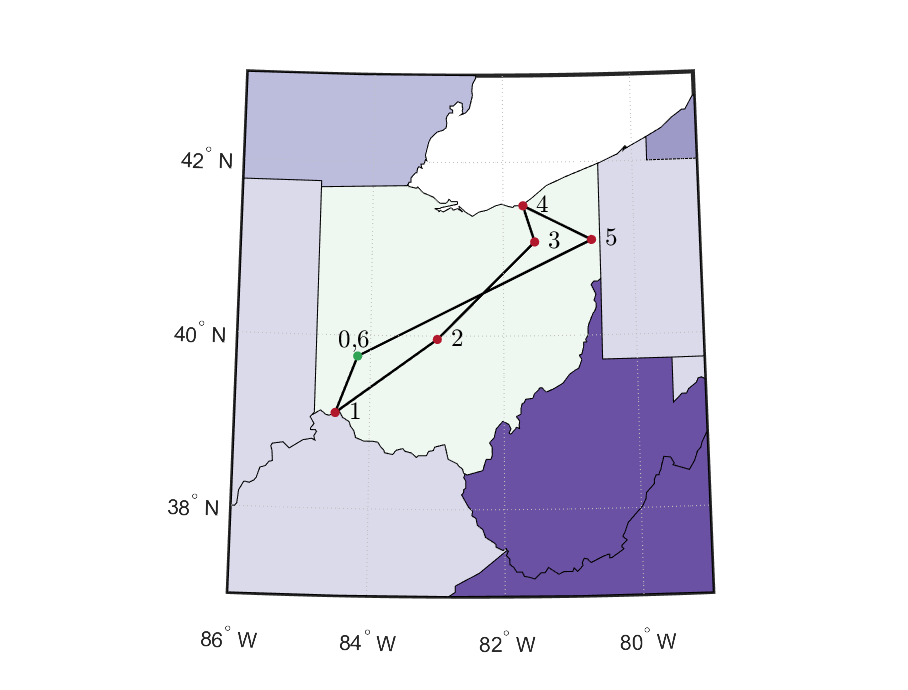
\includegraphics{Thesis/Method_II/fmin1000.eps}
    \caption{Loiter Constrained to at least 1000 lbs of Fuel}
    \label{fig:fmin1000}
\end{figure}
There are several equivalent optimal solutions as the summation of every $F^\tau$ is less than the total fuel available in the aircraft. The addition of a summation over the total fuel consumption while weighting the optimization function to also consider the number of locations visited at each time step will further incentivize the model to seek the most fuel efficient route while loitering for at least 1000 lbs of fuel which is equivalent to loitering for at least ten minutes (varying slightly due to initial weight at each location).\par
Constraining the model further to allow for at least 2200 lbs of fuel burn at each visited location gives a result where not all cities are visited. The path follows the aircraft from Dayton to Cincinnati to Columbus to Youngstown to Akron and back to Dayton. The results are shown in Figure \ref{fig:fmin2200}.
\begin{figure}[h]
    \centering
    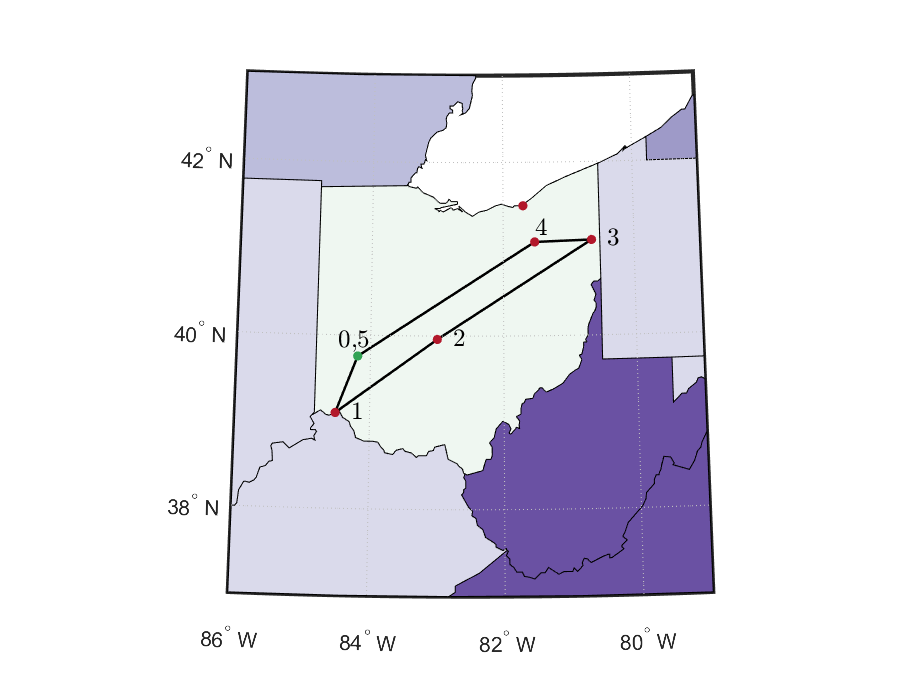
\includegraphics{Thesis/Method_II/fmin2200.eps}
    \caption{Loiter Constrained to at least 2200 lbs of Fuel}
    \label{fig:fmin2200}
\end{figure}
The formulation requires a fuel burn of 2200 lbs at each location which is equivalent to at least 25 minutes of loiter time at each location. The path follows a circular pattern that looks similar to a traveling salesman problem while excluding Cleveland. While Cleveland is closer to the starting location, Youngstown is closer to other interest locations and so the optimization chose a path to Youngstown.\par
Lastly, constraining the model by 3000 lbs of fuel burn at each location demands a loiter time of at least 35 minutes. The results are shown in Figure \ref{fig:fmin3000}.
\begin{figure}[h]
    \centering
    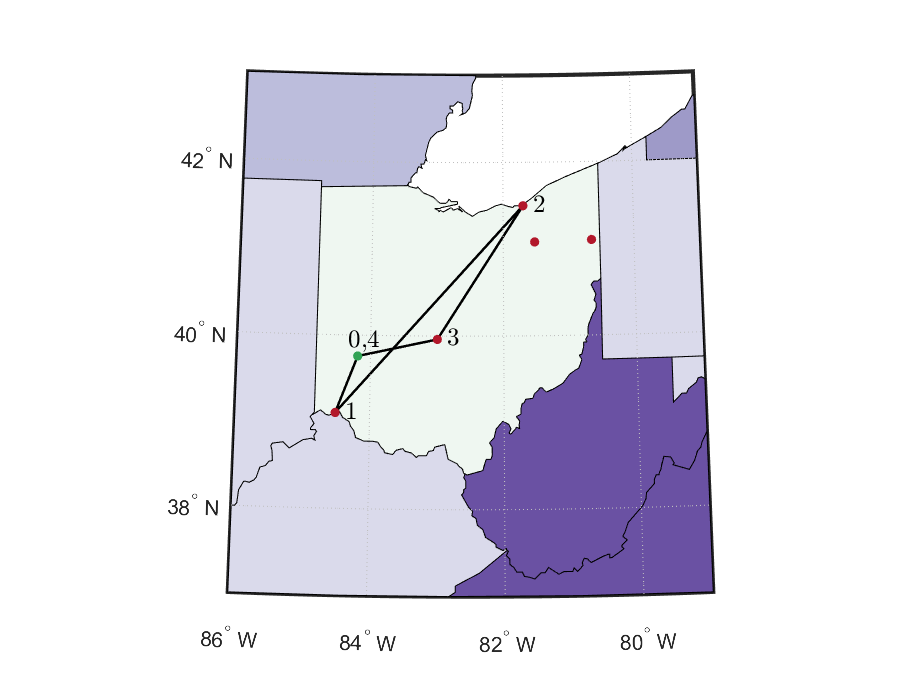
\includegraphics{Thesis/Method_II/fmin3000.eps}
    \caption{Loiter Constrained to at least 3000 lbs of Fuel}
    \label{fig:fmin3000}
\end{figure}
The path shows a more fuel efficient technique where the aircraft's path burns more fuel on its second decision and travels to Cleveland after traveling to Cincinnati in the first decision step. The path is conservative in its third and fourth decision step, traveling to Columbus and then returning to Dayton. Traveling to Akron and Youngstown is considered infeasible with the required loiter time. There are multiple optimal solutions in this scenario as there is still fuel available. Using a weighted optimization technique with an $f_{min}$ at $3000$ lbs to find the most fuel efficient route while visiting the most locations, the objective function becomes
\begin{equation}
    \max \hspace{.5cm} w_1\sum_{\tau\in T}\sum_{i\in I}\sum_{j\in J}x_{ij}^\tau-w_2\sum_{\tau\in T}F^\tau
\end{equation}
where $w_1$ and $w_2$ are arbitrary weights to scale the fuel with the binary location variable. In this example case, $w_1,w_2$ were set to 5000 and 1, respectively. The results are shown in Figure \ref{fig:weightedObj}.
\begin{figure}[h]
    \centering
    \includegraphics{Thesis/Method_II/fmin3000_negF.eps}
    \caption{Weighted Objective Function Result}
    \label{fig:weightedObj}
\end{figure}
The example shows a path from Dayton to Cleveland to Akron to Youngstown. The path chooses a cluster of the closest cities in optimizing the fuel efficiency coupled with visiting the same number of cities as in the previous scenario. Interestingly, the aircraft does not visit Columbus at the end of its path, most likely due to the efficiency of being lighter and cruising farther in the last leg.\par
The use of this technique depends on the objective function and what is desired from the MINLP model and the linear program developed in the previous subsection. The incorporation of aircraft characteristics and parameters allows for a more realistic picture of what path an aircraft could take while meeting certain requirements. 


